% Do not change the options here
\documentclass[bsc,frontabs,parskip,deptreport]{infthesis}

\usepackage{graphicx}
\usepackage[%  
    colorlinks=true,
    pdfborder={0 0 0},
    linkcolor=red,
    citecolor=blue
]{hyperref}


\begin{document}
\begin{preliminary}
\title{A Zoom filter for applause and laughter}

\author{Lasse Wolter}

% to choose your course
% please un-comment just one of the following
%\course{Artificial Intelligence}
\course{Artificial Intelligence and Computer Science}
%\course{Artificial Intelligence and Mathematics}
%\course{Artificial Intelligence and Software Engineering}
%\course{Artificial Intelligence with Management}
%\course{Cognitive Science}
%\course{Computer Science}
%\course{Computer Science and Management Science}
%\course{Computer Science and Mathematics}
%\course{Computer Science and Physics}
%\course{Computer Science with Management}
%\course{Software Engineering}
%\course{Software Engineering with Management}

\project{4th Year Project Report}

\date{\today}

\abstract{

% This skeleton demonstrates how to use the \texttt{infthesis} style for
% undergraduate dissertations in the School of Informatics. It also emphasises the
% page limit, and that you must not deviate from the required style.
% The file \texttt{skeleton.tex} generates this document and can be used as a
% starting point for your thesis. The abstract should summarise your report and
% fit in the space on the first page.
}

\maketitle

\section*{Acknowledgements}


\tableofcontents
\end{preliminary}


% The preliminary material of your report should contain:
% \begin{itemize}
% \item
% The title page.
% \item
% An abstract page.
% \item
% Optionally an acknowledgements page.
% \item
% The table of contents.
% \end{itemize}

\chapter{Introduction}

\chapter{Background}
Automatic applause and laughter detection isn't a new idea. In the following review of existing research we will split applause and laughter detection into different sections. This is due to the fact that very little research includes both kind of detection but rather focus on one of them.

\section{Brief overview of audio processing}

\section{Laughter Detection}
The investigation of the acoustic features of laughter reaches back three decades (\cite{bickley1992acoustic}). The first attempts of laughter detection were done in the early 2000s (\cite{kennedy2004laughter}, \cite{truong2005automatic}). Corpora used in these papers include the ICSI Meeting Recorder corpus \cite{morgan2001meeting}, the CMU, LDC, NIST recordings as well as the Dutch CGN corpus. (TODO: Link overview of existing corpora?). Kennedy and Ellis got the best results using a Mel Frequency Cepstral Coefficients (MFCCs) as features and a Support Vector Machine (SVM) for decision making. 
MFCCs are one of the most widely used features in speech recognition and make use the spectral representation of an audio wave (TODO: link diagram, theory section).
In contrast to Kennedy and Ellis, Truong and Van Leeuwen used Perceptual Linear Prediction (PLP) features with Gaussian Mixture Models (GMM) for classification. We further note that not only the features and predictors differ, also the motivation and definition of laughter events differ. While Kennedy and Ellis define laughter events as 'points in the meeting where more than one person laughs', Truong and Van Leeuwen already considered one person laughing as laughter event. Kennedy and Ellis didn't specify a particular motivation whereas Truong and Van Leeuwen's long-term goal was the investigation of 'paralinguistic events' - laughter is only one of them - to classify the speaker's emotional state.   

Both of these early papers on laughter recognition worked with presegmented laughter samples where predictions only classified a segment as laughter or non-laughter. The determination of segment boundaries of laughter events - which is key for our project - wasn't considered. 

Truong and Leeuwen continued their research and stated that spectral features alone (such as PLP or MFCC) can be used to discriminate between laughter and speech but a significant improvement can be achieved when using prosodic features - features relating the rhythm and intonation (\cite{truong2007automatic}).

Knox and Mirghafori (\cite{knox2006automatic}) were the first to do laughter recognition without presegmented data. They also worked with the ICSI Meeting corpus and used a single layer neural network for classification. Instead of classifying presegmented snippets they classified each 10ms frame using a window of 75 frames around the target frame - 37 before and after the frame (\ref{fig:know_window}). That way an accurate prediction of laughter boundaries of up to 10ms was possible. 
Knox and Mirghafori obtained the best results by combining the output of three NN-systems which used delta MFCCs (derivative of MFCCs), AC PEAK and F0 scores as features, respectively. They achieved an Equal Error Rate (EER) of 7.91\%. They observe that of all tested features MFCCs have the most discriminative power which aligns with prior research by Kennedy and Ellis (\cite{kennedy2004laughter}).

A survey from 2016 (\cite{cosentino2016quantitative}) investigates laughter and laughter detection in different fields up to this point. This survey covers different detection methods, using visual, acoustic and sensory data. For our specific problem we'd like to focus on acoustic data for two reasons. On the one hand people might have privacy concerns if their visual input is used for classification. On the other hand, in video meetings and conferences people often turn off their video input. Consentino et al. also mention the privacy implications of video input and raise the same concern for audio input. Thus, they suggest the use of individual wearable systems to address these concerns. For our project this approach isn't feasible and further, we consider wearable devices as quite intrusive. In our system people can opt-out of using the laughter-detection feature any time. That way people stay in control of their own privacy.
For laughter detection using solely acoustic data, Consentino et al. find that best performance in prior research was obtained using MFCCs and PLPs and combining the resulting classifier with ones that also use prosodic features. This aligns with findings from prior research (\cite{truong2007automatic}, \cite{knox2006automatic}).

More recent research by Gillick et al. (\cite{gillick2021robust}) finds that features learned from spectrograms using deep convolutional networks outperform previous approaches based on MFCCs. Their hypothesis was that models using MFCCs are more prone to pick up surface level characteristics of sound and thus, will be more sensitive to variations like background noise. Gillick et al. expected that features learned using a CNN are more representative of the actual laughter and thus, more robust in different environments. 
Their results suggest that their hypothesis might be correct. The results definitely show that the features learned by a CNN architecture (with or without augmentation) outperform the standard approach using MFCCs. 

\begin{figure}[htp]
    \centering
    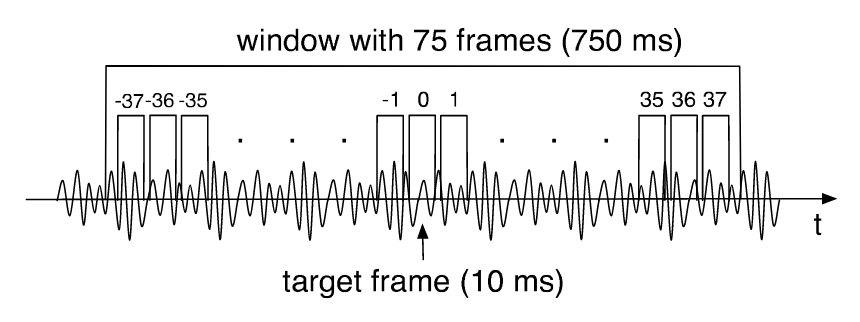
\includegraphics[width=10cm]{imgs/Knox_window.png}
    \caption{Frame window used by Know and Mirghafori}
    \label{fig:know_window}
\end{figure}

\section{Applause}


\bibliographystyle{plain}
\bibliography{mybibfile}

%% You can include appendices like this:
% \appendix
%
% \chapter{First appendix}
%
% \section{First section}
%
% Markers do not have to consider appendices. Make sure that your contributions
% are made clear in the main body of the dissertation (within the page limit).

\end{document}
